\documentclass[11pt,a4paper]{article}
\newcommand{\guideshort}{Beginner quickstart}
% Shared typesetting for the two source-grounded VVE teaching guides.
\usepackage[a4paper,margin=23mm,headheight=15pt]{geometry}
\usepackage{fontspec}
\setmainfont{Liberation Serif}
\setsansfont{Liberation Sans}
\setmonofont{Liberation Mono}
\usepackage{xcolor,graphicx,booktabs,tabularx,longtable,array}
\usepackage{listings,hyperref,tikz}
\usetikzlibrary{arrows.meta,positioning}
\definecolor{vveblue}{HTML}{174A70}
\definecolor{vvelight}{HTML}{F1F5F8}
\definecolor{vvegreen}{HTML}{266547}
\hypersetup{colorlinks=true,linkcolor=vveblue,urlcolor=vveblue,
  pdfauthor={Vienna Vulkan Engine},pdfsubject={Current facade and simple engine; teaching edition}}
\setlength{\parindent}{0pt}
\setlength{\parskip}{6pt plus 1pt}
\setlength{\emergencystretch}{3em}
\sloppy
\renewcommand{\arraystretch}{1.18}
\makeatletter
\def\ps@vve{%
  \def\@oddhead{\small\sffamily Vienna Vulkan Engine\hfil\guideshort}%
  \let\@evenhead\@oddhead
  \def\@oddfoot{\small\sffamily Teaching edition / 16 October 2026\hfil\thepage}%
  \let\@evenfoot\@oddfoot}
\makeatother
\pagestyle{vve}
\lstdefinestyle{vvecpp}{language=C++,basicstyle=\ttfamily\small,
  keywordstyle=\color{vveblue}\bfseries,commentstyle=\color{vvegreen},
  stringstyle=\color{vvegreen},backgroundcolor=\color{vvelight},
  breaklines=true,breakatwhitespace=false,columns=fullflexible,
  keepspaces=true,showstringspaces=false,tabsize=4,
  frame=single,rulecolor=\color{vvelight},framesep=6pt,
  xleftmargin=6pt,xrightmargin=6pt,aboveskip=8pt,belowskip=8pt,
  morekeywords={import,requires,concept,constexpr,consteval,nodiscard}}
\lstset{style=vvecpp}
\newcommand{\api}[1]{{\ttfamily\small\detokenize{#1}}}
\newcommand{\source}[1]{\par\smallskip{\raggedright\footnotesize\sffamily\color{vveblue}Source: \nolinkurl{#1}.\par}}
\newcommand{\lesson}[1]{\clearpage\section{#1}}
\newenvironment{remember}{\begin{quote}\small\textbf{Remember. }}{\end{quote}}
\newenvironment{tryit}{\begin{quote}\small\textbf{Try it. }}{\end{quote}}
\newcommand{\guidecover}[3]{%
  \begin{titlepage}\sffamily\color{vveblue}
  {\large VIENNA VULKAN ENGINE\par}\vspace{20mm}
  {\Huge\bfseries #1\par}\vspace{8mm}
  {\Large #2\par}\vspace{12mm}
  \color{black}{\large #3\par}\vfill
  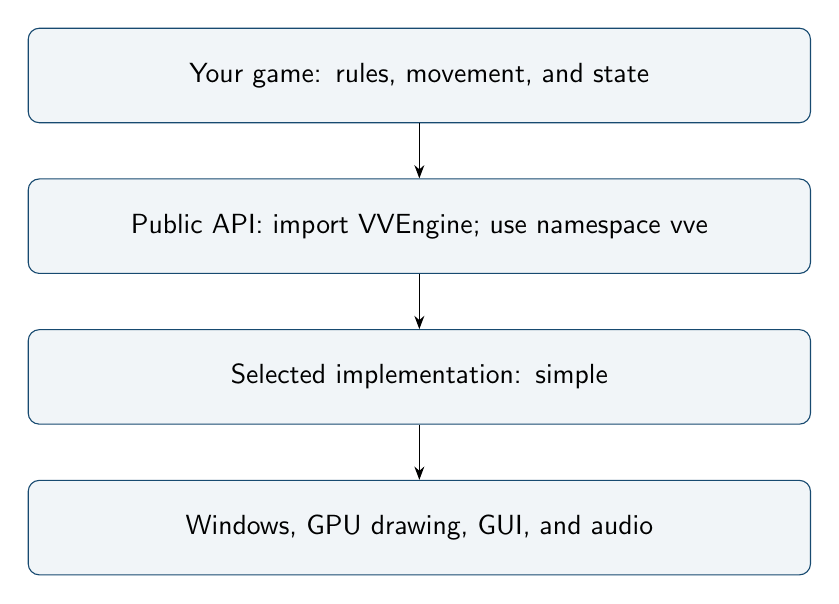
\begin{tikzpicture}[node distance=7mm,every node/.style={draw=vveblue,rounded corners,
    fill=vvelight,text width=0.8\linewidth,align=center,minimum height=12mm,font=\sffamily}]
    \node (game) {Your game: rules, movement, and state};
    \node (facade) [below=of game] {Public API: import VVEngine; use namespace vve};
    \node (engine) [below=of facade] {Selected implementation: simple};
    \node (gpu) [below=of engine] {Windows, GPU drawing, GUI, and audio};
    \draw[-{Stealth}] (game)--(facade);
    \draw[-{Stealth}] (facade)--(engine);
    \draw[-{Stealth}] (engine)--(gpu);
  \end{tikzpicture}\vfill
  {\normalsize Updated 16 October 2026\par}
  {\small Source baseline: 8f875a30; API checked against the local checkout.\par}
  {\small Game code uses the facade. Implementation chapters are for source study.\par}
  \end{titlepage}}

\hypersetup{pdftitle={Vienna Vulkan Engine - beginner quickstart}}
\begin{document}
\guidecover{Your first VVE program}{A short guide for a first project}{You need basic C++: variables, functions, and structs. You do not need to know Vulkan, shaders, or how a game engine works. Start with a supplied example, then build a small program of your own.}

\section*{A route through this guide}
Read sections 1--4 to build the engine and show a scene. Section 5 adds code that runs every frame. The remaining sections explain input, models, the scene tree, GUI images, sound, and common failures. The longer companion, \path{simple_engine_explained.pdf}, explains each idea more slowly and then follows the implementation.

VVE means Vienna Vulkan Engine. Your program calls a public interface called the \emph{facade}. The engine implementation handles the platform and GPU work behind that interface. Write \api{import VVEngine;} and use names beginning with \api{vve::}. Link the engine's CMake target. Both steps are necessary.

\section{Build a supplied example first}
Work from the repository root: the folder containing \path{README.md}, \path{src}, and the build scripts. The first build installs dependencies and may take much longer than later builds. A dependency is another library the engine needs.

\subsection*{Windows: PowerShell}
Install Git, Visual Studio's \emph{Desktop development with C++} workload and CMake tools, and the Vulkan SDK. Use the README's matching compiler/CMake versions for \api{import std}. Bootstrap vcpkg and set \api{VCPKG_ROOT} in your build shell:
\begin{lstlisting}[language={}]
$env:VCPKG_ROOT = 'C:\tools\vcpkg'
.\build_windows.cmd debug
.\bin\debug\exe\simple_forward_demo.exe --frames 120
\end{lstlisting}
The build script sets up the Visual Studio compiler. When using Windows CMake presets directly, use a Developer PowerShell for Visual Studio.

\subsection*{Linux}
Install Ninja, matching Clang, clang-scan-deps, libc++ modules, the Vulkan SDK, and the README's vcpkg dependencies. The script selects a complete installed LLVM toolchain.
\begin{lstlisting}[language={}]
./build_linux.sh debug
./bin/debug/exe/simple_forward_demo --frames 120
\end{lstlisting}

\subsection*{macOS}
Use the README's LLVM, Ninja, Vulkan SDK and KosmicKrisp setup, including its loader manifest.
\begin{lstlisting}[language={}]
./build_macos.sh debug
./bin/debug/exe/simple_forward_demo --frames 120
\end{lstlisting}
\begin{remember}A compiler turns C++ into a program. CMake describes what to build. Ninja runs the build commands. vcpkg installs libraries. The Vulkan SDK supplies the Vulkan tools and Slang shader compiler.\end{remember}
\source{README.md; build_linux.sh; build_macos.sh; build_windows.cmd}

\section{Find the output and understand a failure}
A successful example opens a window and renders a scene. The \api{--frames 120} option makes this supplied example stop after a bounded number of steps. This option is handled by example code; a new program does not automatically understand it.

Debug executables are in \path{bin/debug/exe}; release executables are in \path{bin/release/exe}. Windows adds \api{.exe}. Run from the repository root while learning, so paths such as \path{assets/...} start in the expected folder. A relative filename is relative to the process's working directory, not necessarily the executable's directory.

The build scripts also run tests. Distinguish these stages:
\begin{enumerate}
\item Configuration finds tools and libraries.
\item Compilation checks C++ and builds targets.
\item Linking joins the compiled pieces.
\item Tests run the resulting programs and check their behavior.
\end{enumerate}
Read the first meaningful error in the failing stage. Changing game code will not repair a missing compiler or unsupported graphics driver.

Useful supplied programs include \api{game} for a small game, \api{hierarchy_car} for connected parts, \api{audio_demo} for sound, \api{postprocessing} for image effects, and \api{light_shadow_debug} for a PNG and numerical shadow diagnostics. The \api{sponza} target currently loads the bundled castle scene; the target name does not describe the current asset.

\begin{tryit}Build and run one example without changing its source. Record the command and working directory that succeeded. This gives you a known working starting point.\end{tryit}

\section{Add a small program to the build}
Create \path{examples/mygame/main.cpp}. Put the complete program from the next section in it. Create \path{examples/mygame/CMakeLists.txt}:
\begin{lstlisting}[language={}]
add_executable(mygame main.cpp)
target_link_libraries(mygame PRIVATE
    ViennaVulkanEngine::ViennaVulkanEngine)
vve_set_output_dirs(mygame)
\end{lstlisting}
Add \api{add_subdirectory(mygame)} once to \path{examples/CMakeLists.txt}, then rerun the normal build script. Launch \api{bin/debug/exe/mygame} on Linux/macOS or \api{.\bin\debug\exe\mygame.exe} on Windows.

This layout inherits the repository's C++23 module setup. Do not include an \api{.ixx} file as a header or copy compiler-generated module files by hand. A separate parent CMake project requires additional \api{import std} setup before \api{project()}; use the README when you reach that stage.
\source{src/CMakeLists.txt; examples/CMakeLists.txt; README.md}

\lesson{A complete first program}
This program uses a built-in sample scene. It needs no model or texture file. Copy the whole listing into \path{main.cpp}.
% doc-example: quickstart_scene
\begin{lstlisting}
import std;
import VVEngine;

int main() {
    auto engine = vve::EngineBuilder<>{}
        .applicationName("My first VVE program")
        .addWindow(vve::WindowSetup{}
            .id("main")
            .title("Hello VVE")
            .extent(vve::PixelExtent{800, 600}))
        .build();

    if (const auto result = engine.init(); !result) {
        std::cerr << vve::errorName(result.error()) << '\n';
        return 1;
    }
    auto world = engine.world();
    auto &render = world.get<vve::RenderSystem>();
    if (const auto result = render.loadSampleScene(); !result) {
        std::cerr << vve::errorName(result.error()) << '\n';
        return 2;
    }
    if (const auto result = engine.run(); !result) {
        std::cerr << vve::errorName(result.error()) << '\n';
        return 3;
    }
    return 0;
}
\end{lstlisting}
\textbf{Expected result:} a window containing the sample objects, lit by the sample lights. Close the window to leave \api{run()}.

\api{EngineBuilder<>} collects settings; \api{build()} constructs the engine. The empty angle brackets mean that no game systems are registered yet. A temporary builder moves its systems into the engine; \api{std::move(builder).build()} also supports systems that cannot be copied. A named \api{builder.build()} requires copyable systems. \api{init()} creates the platform windows. GPU rendering begins lazily when a drawable window reaches its first render.

\api{world.get<vve::RenderSystem>()} returns a reference to this engine's renderer. The \api{&} in \api{auto &render} means that the variable refers to the existing object. The engine must stay alive while you use that reference.

A fallible call returns \api{std::expected}: either a value or an error. \api{!result} asks whether it failed. Only use \api{*result} after checking that it succeeded. The first two \api{import} lines make standard-library and VVE declarations available.
\source{src/Engine.ixx; src/World.ixx; src/RenderSystem.ixx}

\lesson{A game system runs your update code}
A \emph{frame} is one trip through the main loop. A \emph{system} is an ordinary C++ object with methods the engine recognizes. Replace \path{main.cpp} with this complete program.
% doc-example: quickstart_system
\begin{lstlisting}
import std;
import VVEngine;

struct Game {
    double elapsed{0.0}; // This value survives between frames.

    auto init(auto &world) -> std::expected<void, vve::Error> {
        return world.template get<vve::RenderSystem>()
            .loadSampleScene();
    }

    void update(auto &world, const vve::FrameContext &frame) {
        elapsed += frame.delta_time.seconds;
        auto &windows = world.template get<vve::WindowSystem>();
        auto input = windows.input();
        if (input.wasKeyPressed(vve::Key::p)) {
            std::cout << "P pressed at " << elapsed << " seconds\n";
        }
    }
};

int main() {
    vve::Engine<Game> engine;
    if (const auto result = engine.run(); !result) {
        std::cerr << vve::errorName(result.error()) << '\n';
        return 1;
    }
    return 0;
}
\end{lstlisting}
The engine owns one \api{Game}. It calls \api{init} during startup and \api{update} after input polling and before rendering. Press P in the focused window to print a message. A key press is a transition; holding P does not repeatedly trigger this branch every frame.

The type of \api{world} is generic because the function uses \api{auto &}. C++ therefore needs \api{template} in \api{world.template get<...>()}. You can copy that spelling without knowing how templates are implemented.

\api{frame.delta_time.seconds} measures elapsed time. Move by \emph{speed multiplied by elapsed seconds}, rather than a fixed distance per frame. The first delta uses \api{DeltaTime{}}: currently 1/60 second.
\source{src/Engine.ixx; src/Types.ixx; src/Window.ixx}

\lesson{Make an object move}
Use \api{RenderObjectHandle} to remember a visible object. A handle is a typed ID, not the object itself. Store it as a member of your system, alongside the position you want.

The following are \textbf{excerpts for a Game system}, not a second complete program. In \api{init}, obtain the renderer, create the cube, and remember its handle:
\begin{lstlisting}
auto &render = world.template get<vve::RenderSystem>();
auto cube = render.addCuboid(
    vve::Vec3{-0.5F, -0.5F, -0.5F},
    vve::Vec3{ 0.5F,  0.5F,  0.5F},
    vve::LinearColor{.value = vve::Vec3{0.2F, 0.7F, 0.3F}});
if (!cube) { return std::unexpected(cube.error()); }
object = *cube; // Game member: vve::RenderObjectHandle object{};
\end{lstlisting}
For an immediately visible teaching object, call \api{setObjectUnlit(object, true)} and check its result. An unlit object shows its colour without needing lights. Set a camera looking at it, or start from the complete moving-cube program in the longer guide.

In \api{update}, obtain input, change your stored transform, and submit the new transform. This version returns an error, so declare the hook to return \api{std::expected<void, vve::Error>}:
\begin{lstlisting}
auto input = world.template get<vve::WindowSystem>().input();
const float dt = static_cast<float>(frame.delta_time.seconds);
if (input.isKeyDown(vve::Key::d)) {
    pose.translation.value.x += 2.0F * dt;
}
// Game member: vve::Transform pose{};
return world.template get<vve::RenderSystem>()
    .setObjectTransform(object, pose);
\end{lstlisting}
At speed 2, a one-second interval produces two world units of movement. VVE does not attach a real-world unit to a coordinate; using one unit as one metre is a useful game convention.

\section{Camera, colour, and the background}
A camera is the view of the scene. These calls belong after obtaining \api{render}:
\begin{lstlisting}
render.setCamera(vve::Camera::lookAt(
    vve::Position{.value = vve::Vec3{0, 3, 7}},
    vve::Position{.value = vve::Vec3{0, 0, 0}}));
render.setBackgroundColor(vve::LinearColor{
    .value = vve::Vec3{0.08F, 0.12F, 0.18F}});
\end{lstlisting}
The sample coordinates use Y as up. A default camera looks along negative Z. Its clipping distances default to 0.1 and 100 world units; objects outside that visible depth interval are clipped. The full guide explains how to fit a camera to a large model.
\source{src/RenderSystem.ixx; src/Types.ixx}

\lesson{Load a model and move its parts}
A \emph{model} is a file containing geometry and often materials and a tree of named parts. Loading it makes source data available. Instantiating it creates visible placements. These are separate steps.

This excerpt assumes \api{world} exists and \api{modelPath} is a \api{std::filesystem::path} naming a real model:
\begin{lstlisting}
auto &assets = world.get<vve::AssetSystem>();
auto &render = world.get<vve::RenderSystem>();
auto scene = assets.loadScene(modelPath);
if (!scene) { return 1; }
auto instance = render.instantiateScene(*scene,
    vve::SceneInstantiationOptions{.keep_hierarchy = true});
if (!instance) { return 2; }
auto root = render.sceneInstanceRoot(*instance);
if (!root) { return 3; }
vve::Transform placement{};
placement.translation.value.x = 3.0F;
if (!render.setNodeTransform(*root, placement)) { return 4; }
\end{lstlisting}
With \api{keep_hierarchy}, the engine copies the model's tree into the world scene tree. Moving the instance root moves the entire model. A wheel node can then move relative to the car. Use \api{sceneInstanceNode} to find the runtime copy of a particular asset node. \api{NodeHandle} and \api{SceneNodeHandle} identify different kinds of node. Reparenting changes transform inheritance, not instance ownership: removing the instance still removes its copied nodes.

To release a level, remove all its placements with \api{render.removeSceneInstance(handle)}, then call \api{assets.unloadScene(sceneHandle)} for each source no longer needed. Check both results. A source with any live placement returns \api{invalid_argument} and remains loaded. Rendering-only cleanup with \api{render.removeScene(source)} retains the imported source data.

Imported lights and cameras are not applied by default. Set your own camera and light, or deliberately enable \api{apply_lights} and \api{apply_cameras} in the instantiation options. An imported model can also be very large or far from the origin; adjust the camera before assuming the import failed.

\section{Textures, sky, sprites, and picking}
\begin{itemize}
\item \api{addTexturedPlane({20,20}, texturePath, {10,10})} creates a 40 by 40 XZ ground plane, repeating the image ten times along each axis.
\item \api{setSkybox(panoramaPath)} shows a 2:1 equirectangular panorama around the camera. Check the returned result.
\item \api{addSprite(size, texturePath)} creates a flat image that turns toward the camera. Transparent pixels allow shaped icons or particles.
\item \api{screenRay(window, normalizedPoint)} builds a ray through a screen location. \api{raycast(origin, direction, distance)} finds the nearest visible object's bounding box along it.
\end{itemize}
These are separate operations. A sprite is a world object; a GUI image is drawn on the interface. The full guide supplies examples and explains opacity and box-based picking.
\source{src/Assets.ixx; src/RenderSystem.ixx; examples/hierarchy_car/hierarchy_car.cpp}

\lesson{Add an interface and optional sound}
\subsection*{A GUI callback}
Include \api{<imgui.h>} before the module imports. Register a callback once; it builds the interface each GUI frame:
\begin{lstlisting}
// Inside Game::init; Game has an int score member.
auto &gui = world.template get<vve::GuiSystem>();
gui.draw([this] {
    ImGui::Begin("Score");
    ImGui::Text("Collected: %d", score);
    ImGui::End();
});
\end{lstlisting}
For a HUD image, call \api{gui.loadImage(path)}, check the returned handle, and retain it. Inside the callback call \api{gui.imageId(handle)}. Draw only when the ID is nonzero: the image may still be waiting for GPU upload. The full guide has a complete recipe.

\subsection*{Sound resources and playing voices}
Audio is optional and opens separately from graphics. This excerpt assumes \api{musicPath} names an existing audio file:
\begin{lstlisting}
auto &audio = world.get<vve::AudioSystem>();
if (!audio.init()) {
    std::cerr << audio.lastError() << '\n';
    return 1;
}
auto sound = audio.loadSound(musicPath,
    vve::AudioLoadMode::on_demand);
if (!sound) { return 2; }
auto voice = audio.play(*sound,
    vve::AudioPlaybackOptions{.loop = true,
        .volume = vve::AudioVolume{.value = 0.4F}});
if (!voice) { return 3; }
\end{lstlisting}
A sound handle identifies reusable loaded data. A playback handle identifies one playing voice. Two \api{play} calls can overlap. Keep \api{*voice} for \api{pause}, \api{resume}, and \api{stop}; check those calls too. Gain is between 0 and 1. \api{on_demand} decodes during playback; it is not disk streaming.

The engine must stay alive during playback. Finished voices are collected during engine steps and before another play call. \api{docs/Audio.md} explains the audio contract and the bundled examples.
\source{src/Gui.ixx; src/Audio.ixx; docs/Audio.md}

\lesson{Troubleshoot one stage at a time}
\begin{tabularx}{\linewidth}{@{}p{0.29\linewidth}X@{}}
\toprule Symptom & First useful check \\\midrule
Compiler or module error & Use the documented compiler, Ninja, and matching standard-library modules. Rebuild through the normal script. \\
Missing dependency & Check the Vulkan SDK and vcpkg installation, triplet, and environment. Read the configure error. \\
Rendering error & Check the returned error from step/run and the failing-stage diagnostic. Recoverable skips do not imply a presented picture. \\
No suitable GPU & Read the rejected-device diagnostic. The simple renderer checks Vulkan 1.3 device features and requests a Vulkan 1.4 instance. \\
Window but no object & Confirm creation and instantiation succeeded. Check visibility, camera, clipping distances, object position, and lighting. \\
File not found & Print the working directory and exact path. Relative paths start at the working directory. \\
Texture remains broken after repair & The simple engine caches decode failures. Clear the scene before retrying that repaired source. \\
No sound & Call \api{audio.init()}; inspect \api{lastError()}, file paths, voice state, and gain. \\
Input seems ignored & Focus the window. An active ImGui widget can claim input. Use held-key queries for continuous movement. \\
Test failure & Read the named CTest result and its output. Build success and test success are different checks. \\
\bottomrule
\end{tabularx}

Run tests again with \api{ctest --test-dir <build-directory> --output-on-failure}. Linux script builds use \path{build/debug-linux}; macOS script builds use \path{build/macos-debug}; Windows script builds use \path{build/debug-windows}. Preset and VS Code build directories can differ.

\subsection*{Where to go next}
Read the longer guide for a complete moving-cube project, ECS-to-render synchronization, local versus world transforms, multiple windows, lighting, GUI images, resource lifetimes, and the CPU-to-GPU path. Use \path{README.md} for platform prerequisites and \path{tests/CMakeLists.txt} for the tests actually registered in your checkout.

\subsection*{Ring Racer's downloaded assets}
The \api{racer} example uses models and sounds from Kenney's \href{https://github.com/KenneyNL/Starter-Kit-Racing}{Starter Kit Racing} and \href{https://github.com/KenneyNL/Starter-Kit-City-Builder}{Starter Kit City Builder}; these assets are CC0. With examples enabled, CMake downloads both kits into the ignored folders \path{assets/racer/kenney/racing} and \path{assets/racer/kenney/city}. The first configure needs internet; later configurations reuse cached downloads and restore missing copies. Texture paths, including \path{models/Textures/colormap.png}, stay intact. See \path{cmake/RacerAssets.cmake} for pinned versions and \path{examples/racer/README.md} for the files used.

\textbf{Edition.} Checked against the local V3 checkout on 17 October 2026. See the companion guide for the detailed validation results.
\source{README.md; src/Engine.ixx; src/Types.ixx; tests/CMakeLists.txt}
\end{document}
